\documentclass[a4paper,11pt]{article}
\usepackage{amsmath,amsthm,amsfonts,amssymb,amscd,amstext,vmargin,graphics,graphicx,tabularx,multicol} 
\usepackage[francais]{babel}
\usepackage[utf8]{inputenc}  
\usepackage[T1]{fontenc} 
\usepackage{pstricks-add,tikz,tkz-tab,variations}
\usepackage[autolanguage,np]{numprint} 

\setmarginsrb{1.5cm}{0.5cm}{1cm}{0.5cm}{0cm}{0cm}{0cm}{0cm} %Gauche, haut, droite, haut
\newcounter{numexo}
\newcommand{\exo}[1]{\stepcounter{numexo}\noindent{\bf Exercice~\thenumexo} : \marginpar{\hfill /#1}}
\reversemarginpar


\newcounter{enumtabi}
\newcounter{enumtaba}
\newcommand{\q}{\stepcounter{enumtabi} \theenumtabi.  }
\newcommand{\qa}{\stepcounter{enumtaba} (\alph{enumtaba}) }
\newcommand{\initq}{\setcounter{enumtabi}{0}}
\newcommand{\initqa}{\setcounter{enumtaba}{0}}

\newcommand{\be}{\begin{enumerate}}
\newcommand{\ee}{\end{enumerate}}
\newcommand{\bi}{\begin{itemize}}
\newcommand{\ei}{\end{itemize}}
\newcommand{\bp}{\begin{pspicture*}}
\newcommand{\ep}{\end{pspicture*}}
\newcommand{\bt}{\begin{tabular}}
\newcommand{\et}{\end{tabular}}
\renewcommand{\tabularxcolumn}[1]{>{\centering}m{#1}} %(colonne m{} centrée, au lieu de p par défault) 
\newcommand{\tnl}{\tabularnewline}

\newcommand{\bmul}[1]{\begin{multicols}{#1}}
\newcommand{\emul}{\end{multicols}}

\newcommand{\trait}{\noindent \rule{\linewidth}{0.2mm}}
\newcommand{\hs}[1]{\hspace{#1}}
\newcommand{\vs}[1]{\vspace{#1}}

\newcommand{\N}{\mathbb{N}}
\newcommand{\Z}{\mathbb{Z}}
\newcommand{\R}{\mathbb{R}}
\newcommand{\C}{\mathbb{C}}
\newcommand{\Dcal}{\mathcal{D}}
\newcommand{\Ccal}{\mathcal{C}}
\newcommand{\mc}{\mathcal}

\newcommand{\vect}[1]{\overrightarrow{#1}}
\newcommand{\ds}{\displaystyle}
\newcommand{\eq}{\quad \Leftrightarrow \quad}
\newcommand{\vecti}{\vec{\imath}}
\newcommand{\vectj}{\vec{\jmath}}
\newcommand{\Oij}{(O;\vec{\imath}, \vec{\jmath})}
\newcommand{\OIJ}{(O;I,J)}


\newcommand{\reponse}[1][1]{%
\multido{}{#1}{\makebox[\linewidth]{\rule[0pt]{0pt}{20pt}\dotfill}
}}

\newcommand{\titre}[5] 
% #1: titre #2: haut gauche #3: bas gauche #4: haut droite #5: bas droite
{
\noindent #2 \hfill #4 \\
#3 \hfill #5

\vspace{-1.6cm}

\begin{center}\rule{6cm}{0.5mm}\end{center}
\vspace{0.2cm}
\begin{center}{\large{\textbf{#1}}}\end{center}
\begin{center}\rule{6cm}{0.5mm}\end{center}
}



\begin{document}
\pagestyle{empty}
\titre{Contrôle sur les chapitres 4, 5 et 6  }{Nom :}{Prénom :}{Classe}{Date}




\textbf{Les exercices avec un 
\includegraphics[scale=0.175]{trefle.eps}  sont à faire sur la copie double.}\\
















\exo{5} 

\initq \q Ranger dans l'ordre décroissant les nombres suivants : \\

$ 5,4$ \hspace*{0.3cm};\hspace*{0.3cm} $ \dfrac{542}{100} + \dfrac{3}{1 000}$ \hspace*{0.3cm} ;\hspace*{0.3cm} $ \dfrac{53}{10} + \dfrac{9}{100}$\hspace*{0.3cm} ; \hspace*{0.3cm}$ 538$ centièmes\hspace*{0.3cm} et\hspace*{0.3cm} $ \dfrac{5470}{1 000}$\\

\reponse[1]\\

\q 	Compléter avec l'un des signes : $ <, > ou =$ \\
 
5,8 . . . 5,08   \hfill   8,04 . . . 8,038   \hfill  8,74 . . . $\dfrac{874}{100}$   \hfill    $\dfrac{7}{10} + \dfrac{4}{100}$ . . . 0,47  \hfill    $12 + \dfrac{9}{100}$   . . . 12,9\\


\q Compléter avec le nombre \textbf{entier} qui suit ou celui qui précède :

\bmul{3}

$12,6 < . . .$

\columnbreak

$6,09 > . . .$

\columnbreak

$ . . . < \dfrac{2 453 }{100}$

\emul

\exo{2,5} 

\initq \q Intercaler un nombre entre 3,1 et 3,2 : \\
\reponse[1]

\q Encadrer les nombres suivants par deux entiers consécutifs :

\bmul{2}

. . . . . . . < 74,586 < . . . . . . .

\columnbreak

. . . . . . . < $ \dfrac{8523}{100}$ < . . . . . . .


\emul


\exo{3} 
\includegraphics[scale=0.175]{trefle.eps}\\
$\pi$ est un nombre qui a fasciné tant de savants depuis l'antiquité. \\
$\pi$ est un nombre irrationnel (c'est à dire qu'il s'écrit avec un nombre infini de décimales sans suite logique). \\
Le 2 Août 2010, 5 000 milliards de décimales de $\pi$ ont été découverts par deux japonnais Alexander J. Yee et Shigeru en 90 jours.\\
 Et 1 an plus tard après 371 jours de travail, ces même chercheurs ont battu leur record et ont découvert jusqu'à 10 000 milliards de décimales de $\pi$. En voici une toute petite approximation :

\begin{center}
$\pi \approx 3.141 592 653 589 793 238 462 643 383 279 502 884 197 169 399 375 $
\end{center}



\initq \q Encadrer le nombre $\pi$ au millième près.\\


\q Donner la valeur approchée au millième près de $\pi$ par défaut.\\



\q Encadrer le nombre $\pi$ au dixième près.\\


\q Donner la valeur approchée au dixième près de $\pi$ par excès.\\


\exo{3}

\includegraphics[scale=0.8]{demidroite.eps} 


\initq \q Donner les abscisses des points A, B et C : \reponse[1]\\


\q Placer (à l'aide d'une croix bleue) les points E, F et G sur la demi-droite graduée :

\begin{center}
 E(2)  ;  F(5,6)   et   G(quatre-vingts centièmes)
\end{center}


\exo{1,5} Pour chaque question, entourer la bonne réponse :\\

\begin{flushleft}
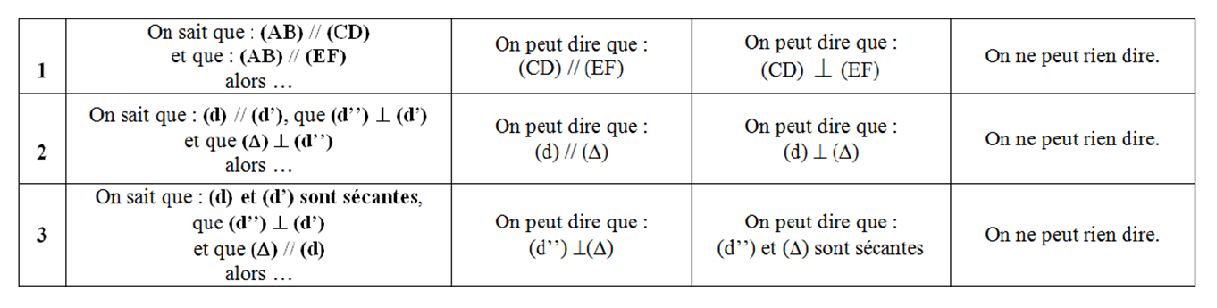
\includegraphics[scale=0.85]{qcm.eps} 
\end{flushleft}


\exo{3,75} 
\includegraphics[scale=0.175]{trefle.eps}\\

\initq \q Avec la règle plate et l'équerre, construire soigneusement sur votre copie double :

\bi

\item Tracer une droite (AL)

\item Placer un point $M \in (AC)$ et un point $B \notin (AC)$

\item Tracer la droite $ (d_{1})$ perpendiculaire à la droite (AL) passant par le point M
 
\item Tracer la droite $ (d_{2})$ parallèle à la droite (AM) passant par le point B.\\

\ei

\q Démontrer que les droites $ (d_{1})$ et $ (d_{2})$ sont perpendiculaires.\\

\exo{1.25} 
\includegraphics[scale=0.175]{trefle.eps}\\

\bmul{2}



Luc doit construire la figure ci-contre. \\
Voici les différentes instructions dans le désordre. \\
\textbf{Réécrire sur votre copie double} les instructions dans le bon ordre.\\

\columnbreak

\includegraphics[scale=0.9]{programmeconstruction.eps} 


\emul

\bi	
\item Tracer la droite perpendiculaire à (MU) passant par I. Elle coupe (MU) en O.
\item Tracer la droite perpendiculaire à (MA) passant par U. Elle coupe (MA) en I.
\item Les droites (OH) et (IU) sont sécantes en B.
\item Tracer un triangle MAU.
\item Tracer la droite parallèle à (MA) passant par O. Elle coupe (AU) en H.\\
\ei

\exo{}BONUS\\

\includegraphics[scale=0.6]{garam.eps} \hspace*{2cm} 
\includegraphics[scale=1]{carremagiquue.eps}  



\end{document}
